\documentclass[11pt]{article}

% ------------------------------------------------------------------ preamble
\usepackage[a4paper,margin=2.4cm]{geometry}
\usepackage{amsmath,amssymb,amsthm}
\usepackage{booktabs}
\usepackage{multirow}
\usepackage{graphicx}
\usepackage{xcolor}
\usepackage{siunitx}
\usepackage{caption}
\usepackage[hidelinks]{hyperref}
\usepackage{enumitem}

\graphicspath{{../figures/}}
\sisetup{group-separator={,},group-minimum-digits=4}

\definecolor{navy}{HTML}{1F3B73}
\definecolor{brick}{HTML}{B3331A}
\hypersetup{colorlinks=true,linkcolor=navy,urlcolor=navy,citecolor=navy}

\newtheorem{definition}{Definition}
\newcommand{\VaR}{\operatorname{VaR}}
\newcommand{\ES}{\operatorname{ES}}
\newcommand{\PR}{\mathbb{P}}
\newcommand{\E}{\mathbb{E}}

\title{\textbf{Monte Carlo Simulation for Tail Risk}\\[2pt]
\large Calibration, Simulation, and the Gap with Reality}
\author{venkat}
\date{\today}

% ------------------------------------------------------------------ document
\begin{document}
\maketitle

\begin{abstract}
\noindent These are working notes on understanding \emph{tail risk} through
Monte Carlo simulation. The guiding question is the relationship between
\textbf{calibration} (fitting a model to data we have seen) and
\textbf{reality} (the losses the world actually delivers). I build a dataset
from a known fat-tailed, volatility-clustering process, calibrate three risk
models to it (Normal, Student-$t$, and an Extreme-Value/Generalized-Pareto
tail model), estimate Value-at-Risk and Expected Shortfall by Monte Carlo,
and then \emph{backtest} each calibration against the realised series. The
recurring lesson: a model can fit the body of the data and still be dangerously
wrong in the tail, and calibration only ever recovers the model you assumed ---
not necessarily the process that generated the world.
\end{abstract}

\tableofcontents
\medskip
\hrule

% ===================================================================
\section{The question}
A risk number is a claim about the future stated as a probability. When we say
``the one-day 99\% Value-at-Risk is 3.2\%,'' we are asserting that a loss worse
than 3.2\% should happen on about one day in a hundred. Two separate things must
go right for that claim to hold:
\begin{enumerate}[nosep]
  \item \textbf{Calibration} --- we picked model parameters that match the data.
  \item \textbf{Specification} --- the model \emph{family} is capable of
        describing reality in the first place.
\end{enumerate}
Calibration is an optimisation problem and always ``succeeds'': it returns the
best parameters \emph{within the family you chose}. Whether those parameters
say anything true about the world is a different question, answered only by
confronting the model with out-of-sample reality. These notes make that
distinction concrete and measurable.

% ===================================================================
\section{Tail risk: VaR and Expected Shortfall}
Let $L$ denote the loss over the risk horizon (here, one day), so that
$L=-r$ for a log-return $r$. Fix a confidence level $\alpha\in(0,1)$
(e.g.\ $0.99$).

\begin{definition}[Value-at-Risk]
$\VaR_\alpha(L)$ is the $\alpha$-quantile of the loss distribution,
\[
   \VaR_\alpha(L) \;=\; \inf\{\,\ell\in\mathbb{R} : \PR(L\le \ell)\ge \alpha\,\}.
\]
\end{definition}

\noindent VaR answers ``how bad is a bad day, at the $\alpha$ threshold?''
It says nothing about \emph{how much worse} the rare day beyond the threshold
can be, and it is not sub-additive --- diversification can appear to
\emph{increase} it. The fix is the conditional average of the tail:

\begin{definition}[Expected Shortfall]
\[
   \ES_\alpha(L) \;=\; \frac{1}{1-\alpha}\int_\alpha^1 \VaR_u(L)\,\mathrm{d}u
   \;=\; \E\!\left[\,L \mid L \ge \VaR_\alpha(L)\,\right]
   \quad(\text{for continuous } L).
\]
\end{definition}

\noindent ES (a.k.a.\ CVaR or TVaR) is \emph{coherent}: monotone, translation
invariant, positively homogeneous, and sub-additive. It is the average loss on
the worst $(1-\alpha)$ fraction of days, and it is the quantity post-2016
Basel rules put at the centre of market-risk capital. Both VaR and ES depend
entirely on the \emph{shape of the tail} --- which is exactly the part of the
distribution that data is sparsest about.

% ===================================================================
\section{The data and its stylised facts}
To study calibration against a known truth, I generate \num{3000} daily
log-returns ($\approx$12 trading years) from a $\mathrm{GARCH}(1,1)$ process
with standardised Student-$t$ innovations:
\[
  r_t = \mu + \sigma_t z_t,\qquad
  \sigma_t^2 = \omega + a\,\varepsilon_{t-1}^2 + b\,\sigma_{t-1}^2,\qquad
  z_t \sim t_\nu(\text{unit variance}),
\]
with true parameters $\mu=\num{5e-4}$, $\omega=\num{2e-6}$, $a=0.08$,
$b=0.90$, and $\nu=4$. This process is the ``reality'' in the experiment. It
reproduces the two stylised facts that make tail risk hard:

\begin{description}[leftmargin=1.4em,nosep]
  \item[Fat tails.] The realised series has excess kurtosis $\approx 23.7$
        (Gaussian $=0$): extreme moves are vastly more frequent than a Normal
        allows.
  \item[Volatility clustering.] Variance is persistent ($a+b=0.98$): turbulent
        days follow turbulent days. Figure~\ref{fig:returns} shows the bursts.
\end{description}

\begin{figure}[h]
  \centering
  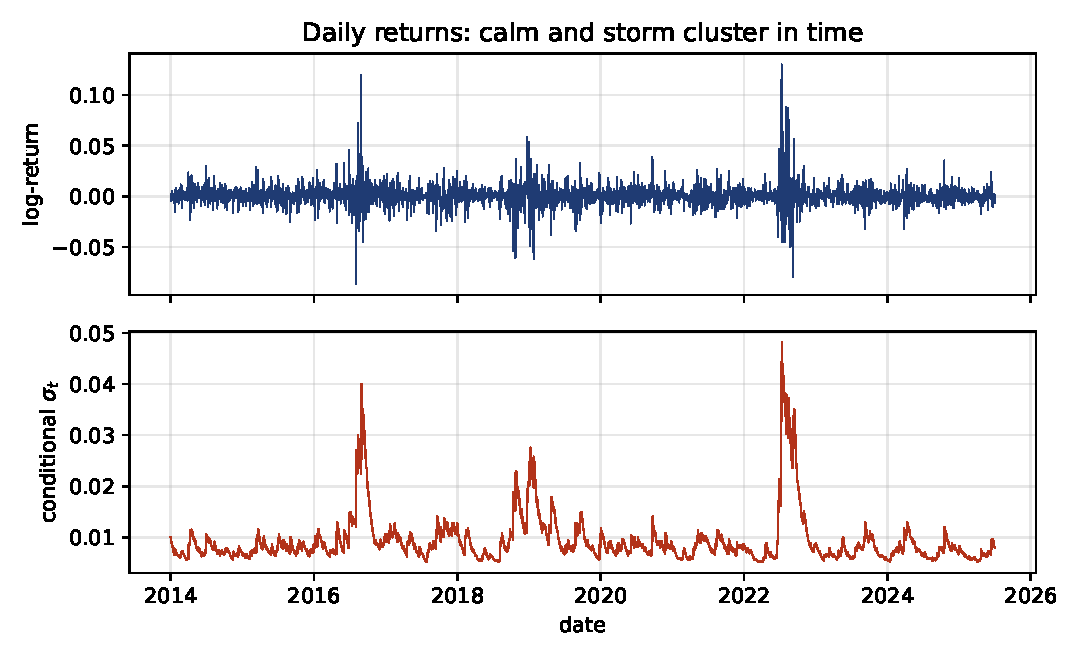
\includegraphics[width=\textwidth]{fig_returns.pdf}
  \caption{Top: simulated daily returns. Bottom: the latent conditional
  volatility $\sigma_t$. Large moves and high volatility cluster --- they are
  not sprinkled uniformly through time.}
  \label{fig:returns}
\end{figure}

\noindent A Normal QQ-plot (Figure~\ref{fig:qq}) is the quickest diagnostic:
if the data were Gaussian the points would lie on the line; instead the tails
peel away, the signature of a heavy-tailed law.

\begin{figure}[h]
  \centering
  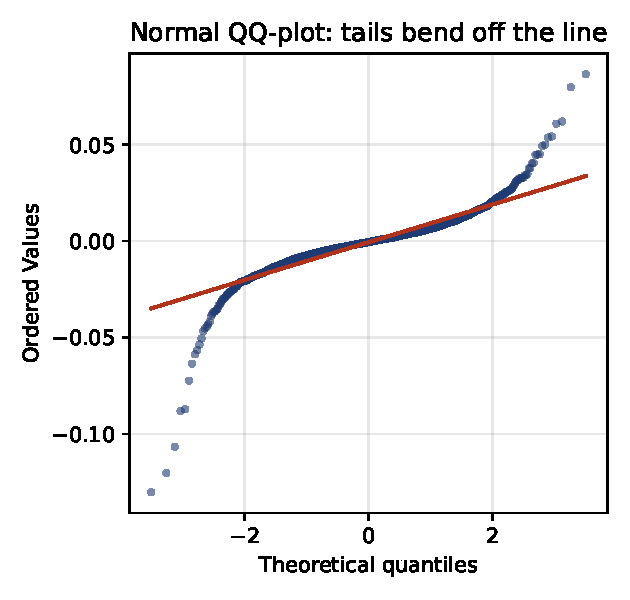
\includegraphics[width=0.52\textwidth]{fig_qq.pdf}
  \caption{Normal QQ-plot of the losses. The systematic departure at both ends
  is the visual fingerprint of fat tails.}
  \label{fig:qq}
\end{figure}

% ===================================================================
\section{Calibration: three models}
I fit three models to the loss series $L=-r$ by maximum likelihood, in order of
increasing tail-awareness.

\paragraph{Normal.} Two parameters $(\mu,\sigma)$, fit by the sample mean and
standard deviation. Convenient, closed-form everything, and thin-tailed by
construction --- the null hypothesis we expect to fail.

\paragraph{Student-$t$.} Adds a degrees-of-freedom parameter $\nu$ that fattens
the tails; as $\nu\to\infty$ it collapses to the Normal. Fit by MLE over
$(\nu,\text{loc},\text{scale})$.

\paragraph{Extreme Value Theory (Peaks-Over-Threshold).} Instead of modelling
the whole distribution, EVT models \emph{only} the tail. The
Pickands--Balkema--de Haan theorem says that for a high threshold $u$, the
exceedances $L-u\mid L>u$ converge to a Generalized Pareto Distribution (GPD):
\[
  G_{\xi,\beta}(y) = 1-\Big(1+\tfrac{\xi y}{\beta}\Big)^{-1/\xi},\qquad y>0.
\]
The shape $\xi>0$ signals a heavy (power-law) tail. I set $u$ at the 90\%
quantile, leaving \num{300} exceedances, and fit $(\xi,\beta)$ by MLE.

\begin{table}[h]
  \centering
  \caption{Calibrated parameters (loss space).}
  \label{tab:params}
  \begin{tabular}{llll}
    \toprule
    Model & \multicolumn{3}{l}{Parameters}\\
    \midrule
    Normal      & $\mu=-0.00063$ & $\sigma=0.01080$ & \\
    Student-$t$ & $\nu=2.21$     & loc$=-0.00062$    & scale$=0.00536$\\
    GPD (POT)   & $u=0.0094$     & $\xi=+0.260$      & $\beta=0.00598$\\
    \bottomrule
  \end{tabular}
\end{table}

\paragraph{A first surprise --- calibration $\ne$ truth.}
The true \emph{conditional} innovation has $\nu=4$, yet the calibrated i.i.d.\
Student-$t$ reports $\nu\approx 2.21$. This is not an error; it is the central
lesson appearing early. Mixing many days of \emph{different} volatilities (the
GARCH effect) produces an \emph{unconditional} distribution with much heavier
tails than any single conditional $t_4$. Fitting an i.i.d.\ model to a
clustered reality forces $\nu$ down to absorb that extra kurtosis. The number
that ``best fits'' is faithful to the \emph{assumed family}, not to the
mechanism that generated the data. Figure~\ref{fig:density} shows the cost of
the thin-tailed assumption directly.

\begin{figure}[h]
  \centering
  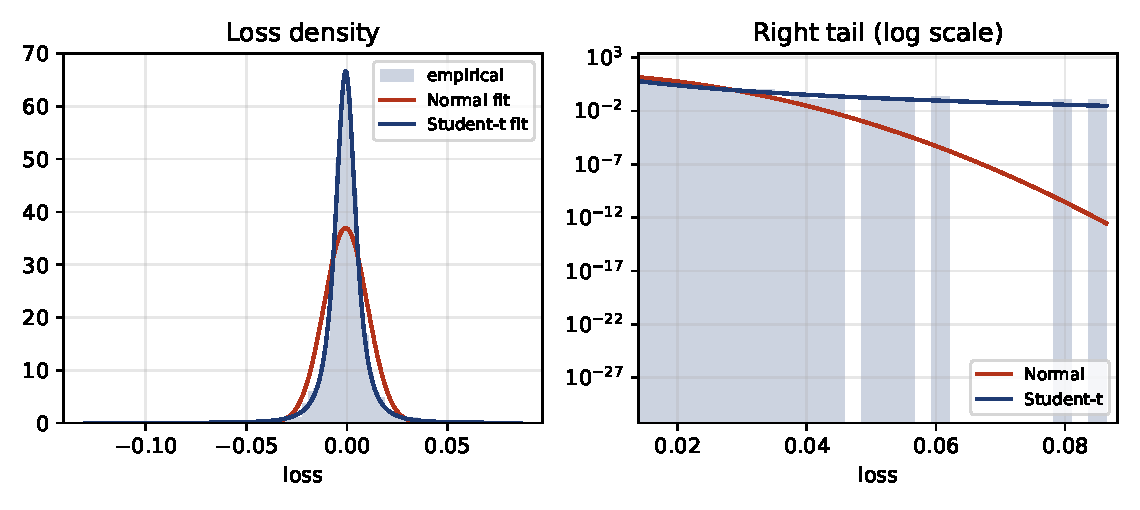
\includegraphics[width=\textwidth]{fig_density.pdf}
  \caption{Left: loss histogram with the Normal and Student-$t$ fits. Right:
  the same right tail on a log scale. The Normal (red) plunges to zero; the
  Student-$t$ (navy) keeps mass out where the real losses live.}
  \label{fig:density}
\end{figure}

% ===================================================================
\section{Monte Carlo simulation}
For the Normal and Student-$t$ fits, VaR and ES have closed forms. Real
portfolios --- options, path-dependence, many coupled risk factors --- usually
do not. Monte Carlo is the general method:

\begin{enumerate}[nosep]
  \item Draw $N$ i.i.d.\ losses $L^{(1)},\dots,L^{(N)}$ from the calibrated model.
  \item Estimate $\widehat{\VaR}_\alpha$ as the empirical $\alpha$-quantile.
  \item Estimate $\widehat{\ES}_\alpha$ as the mean of the draws
        $\ge \widehat{\VaR}_\alpha$.
\end{enumerate}

The estimator carries \emph{sampling noise} of order $1/\sqrt{N}$. For a
quantile, the asymptotic standard error is
\[
  \operatorname{s.e.}(\widehat{\VaR}_\alpha)\;\approx\;
  \frac{1}{f(\VaR_\alpha)}\sqrt{\frac{\alpha(1-\alpha)}{N}},
\]
which blows up as $\alpha\to1$ (the density $f$ in the tail is tiny). Tail
quantiles are intrinsically the hardest to simulate --- precisely why variance
reduction and EVT exist. Figure~\ref{fig:mc} shows convergence to the analytic
value.

\begin{figure}[h]
  \centering
  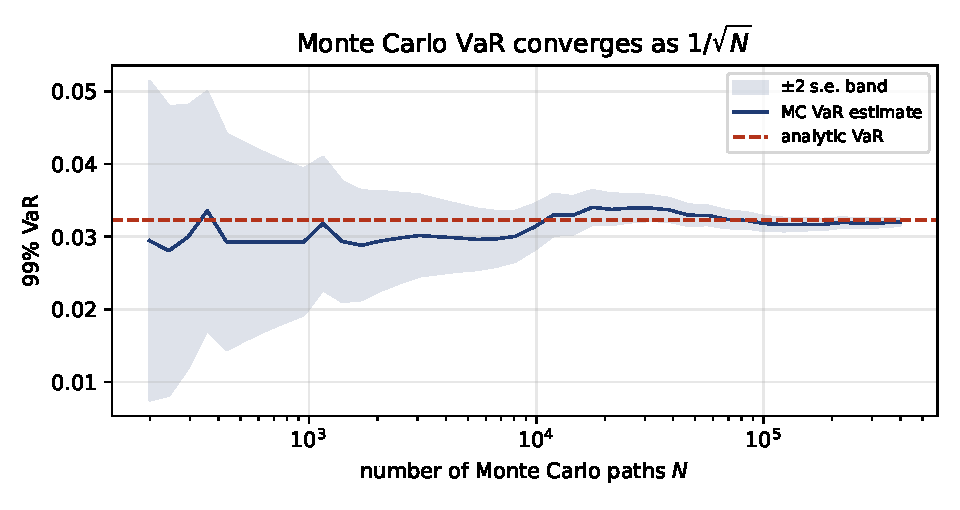
\includegraphics[width=0.82\textwidth]{fig_mc_converge.pdf}
  \caption{Monte Carlo 99\% VaR versus number of paths $N$, with a
  $\pm 2$ standard-error band, converging to the closed-form value (dashed).}
  \label{fig:mc}
\end{figure}

\begin{table}[h]
  \centering
  \caption{Monte Carlo ($N=\num{200000}$) vs.\ closed form, calibrated
  Student-$t$. Agreement here validates the \emph{simulation}; it says nothing
  about whether the model is \emph{right}.}
  \label{tab:mc}
  \begin{tabular}{lcccc}
    \toprule
    & \multicolumn{2}{c}{$\alpha=95\%$} & \multicolumn{2}{c}{$\alpha=99\%$}\\
    \cmidrule(lr){2-3}\cmidrule(lr){4-5}
    & VaR & ES & VaR & ES\\
    \midrule
    Monte Carlo & $0.0141$ & $0.0279$ & $0.0326$ & $0.0597$\\
    Analytic    & $0.0141$ & $0.0280$ & $0.0323$ & $0.0603$\\
    \bottomrule
  \end{tabular}
\end{table}

% ===================================================================
\section{Calibration versus reality: backtesting}
This is the heart of the matter. Each calibrated model emits a VaR. Reality ---
the \num{3000} realised days --- emits actual losses. A \emph{breach} is a day
on which the realised loss exceeds the model's VaR. At level $\alpha$ we expect
breaches on a $(1-\alpha)$ fraction of days. We test that with the Kupiec
proportion-of-failures likelihood-ratio statistic
\[
  LR_{\text{POF}} = -2\ln\!\frac{(1-p)^{\,n-x}\,p^{\,x}}
        {(1-\hat\pi)^{\,n-x}\,\hat\pi^{\,x}}
  \;\xrightarrow{\;H_0\;}\;\chi^2_1,
  \qquad \hat\pi=\tfrac{x}{n},\; p=1-\alpha,
\]
where $x$ is the breach count over $n$ days. A small $p$-value means the
observed breach rate is inconsistent with the claimed level.

\begin{table}[h]
  \centering
  \caption{Backtest over $n=\num{3000}$ realised days. The Normal model is
  \textcolor{brick}{rejected} at both levels; the fat-tailed models pass.}
  \label{tab:backtest}
  \begin{tabular}{llccccc}
    \toprule
    $\alpha$ & Model & VaR & Breaches & Expected & Kupiec $p$ & Verdict\\
    \midrule
    \multirow{3}{*}{95\%}
      & Normal      & 0.0171 & 100 & 150.0 & 0.000 & \textcolor{brick}{REJECT}\\
      & Student-$t$ & 0.0141 & 148 & 150.0 & 0.867 & PASS\\
      & GPD/EVT     & 0.0139 & 150 & 150.0 & 1.000 & PASS\\
    \midrule
    \multirow{3}{*}{99\%}
      & Normal      & 0.0245 &  42 &  30.0 & 0.038 & \textcolor{brick}{REJECT}\\
      & Student-$t$ & 0.0323 &  23 &  30.0 & 0.180 & PASS\\
      & GPD/EVT     & 0.0283 &  29 &  30.0 & 0.854 & PASS\\
    \bottomrule
  \end{tabular}
\end{table}

\noindent Read the Normal row carefully, because it shows \emph{two opposite
failures of the same model}:
\begin{itemize}[nosep]
  \item At 95\% it is \emph{too conservative} (100 breaches vs.\ 150): its wide
        ``body'' overstates ordinary risk and wastes capital.
  \item At 99\% it is \emph{too reckless} (42 breaches vs.\ 30): its thin tail
        understates extreme risk --- the failure that bankrupts you.
\end{itemize}
A single mis-specified family is simultaneously charging too much for calm and
too little for catastrophe. Figure~\ref{fig:breaches} marks where reality broke
through the 99\% lines.

\begin{figure}[h]
  \centering
  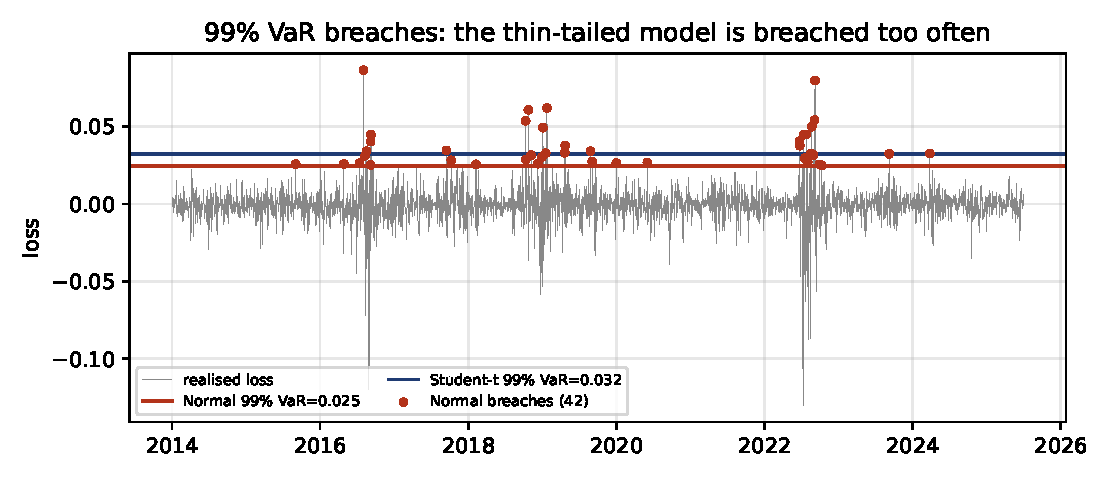
\includegraphics[width=\textwidth]{fig_breaches.pdf}
  \caption{Realised losses with each model's 99\% VaR. Red dots are days that
  breached the Normal VaR --- visibly clustered, another reminder that breaches
  arrive together, not independently.}
  \label{fig:breaches}
\end{figure}

\subsection{Counting is not enough: the independence test}
Kupiec asks \emph{how many} breaches occurred. It is blind to \emph{when}. A
model that breaches 150 times in 3{,}000 days passes it perfectly --- even if
all 150 fell in three bad months. That matters: a desk that loses its VaR
several days running is in far more trouble than one that loses it on scattered
days, and a GARCH reality produces exactly that pattern.

Christoffersen's test fits a two-state Markov chain to the 0/1 breach sequence.
Let $n_{ij}$ count days in state $j$ following a day in state $i$ (1 = breach),
and set
\[
  \hat\pi_{01}=\frac{n_{01}}{n_{00}+n_{01}},\qquad
  \hat\pi_{11}=\frac{n_{11}}{n_{10}+n_{11}},\qquad
  \hat\pi=\frac{n_{01}+n_{11}}{n_{00}+n_{01}+n_{10}+n_{11}}.
\]
$\hat\pi_{11}$ is the breach rate on the day \emph{after} a breach. Under
independence it equals $\hat\pi_{01}$, and
\[
  LR_{\text{ind}} = -2\ln\!\frac{(1-\hat\pi)^{\,n_{00}+n_{10}}\,\hat\pi^{\,n_{01}+n_{11}}}
     {(1-\hat\pi_{01})^{\,n_{00}}\,\hat\pi_{01}^{\,n_{01}}\,
      (1-\hat\pi_{11})^{\,n_{10}}\,\hat\pi_{11}^{\,n_{11}}}
  \;\xrightarrow{\;H_0\;}\;\chi^2_1 .
\]
The sum $LR_{\text{cc}}=LR_{\text{POF}}+LR_{\text{ind}}\sim\chi^2_2$ tests
count and timing jointly (``conditional coverage'').

\begin{table}[h]
  \centering
  \caption{Independence of breaches. At 95\% \textcolor{brick}{every} model is
  rejected --- including the two that passed Kupiec.}
  \label{tab:christoffersen}
  \begin{tabular}{llcccc}
    \toprule
    $\alpha$ & Model & Kupiec $p$ & $\hat\pi_{11}$ & $\hat\pi_{01}$ & Christoffersen $p$\\
    \midrule
    \multirow{3}{*}{95\%}
      & Normal      & 0.000 & 11.0\% & 3.1\% & \textcolor{brick}{0.000}\\
      & Student-$t$ & 0.867 & 14.2\% & 4.5\% & \textcolor{brick}{0.000}\\
      & GPD/EVT     & 1.000 & 14.0\% & 4.5\% & \textcolor{brick}{0.000}\\
    \midrule
    \multirow{3}{*}{99\%}
      & Normal      & 0.038 & 7.1\%  & 1.3\% & \textcolor{brick}{0.022}\\
      & Student-$t$ & 0.180 & 0.0\%  & 0.8\% & 0.551\\
      & GPD/EVT     & 0.854 & 3.4\%  & 0.9\% & 0.286\\
    \bottomrule
  \end{tabular}
\end{table}

\noindent At 95\%, a breach triples the chance of another the next day. Fixing
the tail \emph{shape} (Student-$t$, EVT) fixed the \emph{count}; it did nothing
for the \emph{timing}, because every model here is unconditional --- one VaR
number for calm and storm alike. The 99\% passes deserve suspicion rather than
comfort: with only 23--29 breaches, just 0--1 of them fall on consecutive days,
so the test has almost no power and the $\chi^2$ approximation is rough. A pass
there means ``not enough evidence of clustering,'' not ``independent.''

% ===================================================================
\section{The fix: a VaR that moves with volatility}
Every model so far answers ``how fat is the tail?'' and ignores ``how stormy
is today?''. GARCH-filtered EVT (McNeil and Frey, 2000) answers the two
questions separately.
\begin{enumerate}[nosep,leftmargin=1.6em]
  \item \textbf{GARCH(1,1) for the storm.} Fit
        $\sigma_t^2=\omega+\alpha\,\varepsilon_{t-1}^2+\beta\,\sigma_{t-1}^2$
        by Gaussian quasi-maximum likelihood. The Normal likelihood still gives
        consistent GARCH parameters when the true shocks are fat-tailed. It
        is only wrong about the tail, which step 2 handles instead.
        $\sigma_t$ uses information up to day $t-1$ only.
  \item \textbf{EVT for the tail.} Standardise,
        $z_t=(r_t-\mu)/\sigma_t$. With the clustering divided out, the $z_t$
        are close to i.i.d., so fitting a POT--GPD to their loss tail is now
        well posed. It gives a fixed tail quantile $q_z(p)$.
  \item \textbf{Recombine.} $\mathrm{VaR}_t(p)=-\mu+\sigma_t\,q_z(p)$: a
        fixed tail shape scaled by a moving volatility.
\end{enumerate}

\begin{table}[h]
  \centering
  \caption{GARCH-EVT against the best unconditional model. It is the only
  model that passes both tests at both levels.}
  \label{tab:garchevt}
  \begin{tabular}{llcccccc}
    \toprule
    $\alpha$ & Model & mean VaR & Breaches & Kupiec $p$ & $\hat\pi_{11}$ & $\hat\pi_{01}$ & Christoffersen $p$\\
    \midrule
    \multirow{2}{*}{95\%}
      & Student-$t$ & 0.0141 & 148 & 0.867 & 14.2\% & 4.5\% & \textcolor{brick}{0.000}\\
      & GARCH-EVT   & 0.0139 & 151 & 0.933 & 6.0\%  & 5.0\% & 0.603\\
    \midrule
    \multirow{2}{*}{99\%}
      & Student-$t$ & 0.0323 & 23  & 0.180 & 0.0\%  & 0.8\% & 0.551\\
      & GARCH-EVT   & 0.0247 & 28  & 0.711 & 0.0\%  & 0.9\% & 0.468\\
    \bottomrule
  \end{tabular}
\end{table}

\noindent At 95\%, the day after a breach now carries a 6.0\% breach rate against
a 5.0\% base, where the static models showed 14\% against 4.5\%. The
clustering is gone (Figure~\ref{fig:conditional}). The capital story is just as
important. At 99\%, GARCH-EVT holds \emph{less} VaR on average than the
Student-$t$ (0.0247 against 0.0323) and still delivers the right breach
count. It holds less in calm periods and more in storms, where the static model
holds the same amount everywhere and so over-reserves in calm and under-reserves in crisis.

\begin{figure}[h]
  \centering
  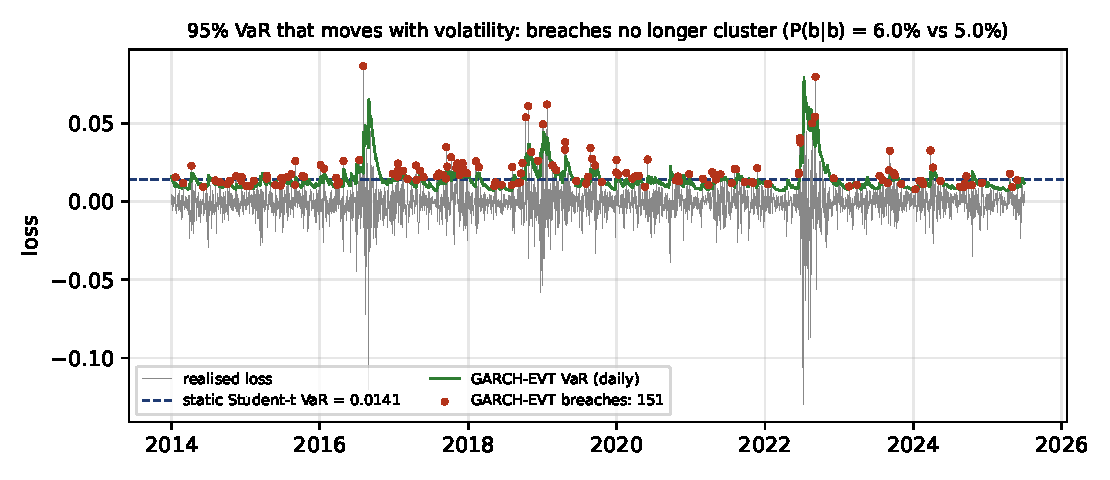
\includegraphics[width=\textwidth]{fig_conditional.pdf}
  \caption{GARCH-EVT 95\% VaR (green) rises into the 2016 and 2022 storms and
  relaxes after them. Its breaches are spread across the sample instead of
  bunched into the volatile spells.}
  \label{fig:conditional}
\end{figure}

\paragraph{Checks that the pieces behave.}
\begin{itemize}[nosep]
  \item \emph{GARCH recovers the truth.} $\hat\alpha=0.097$, $\hat\beta=0.888$,
        against a true $0.08$ and $0.90$. When the model family matches reality,
        calibration finds reality. Contrast the unconditional $\hat\nu=2.21$
        against a true $4$.
  \item \emph{Filtering removes the clustering.} Excess kurtosis falls from
        23.7 on raw returns to 4.5 on the residuals. What remains is the
        genuine fat tail of the $t_4$ shocks.
  \item \emph{The residual tail index is biased low, as expected.} The fit gives
        $\hat\xi=0.12$, where a $t_4$ tail has $\xi=1/4$. This is not a bug.
        A Student-$t$ tail is Pareto only asymptotically, so a GPD fitted
        above a moderate threshold underestimates $\xi$. On two million clean
        $t_4$ draws the same procedure gives $\hat\xi\approx0.17$ at the 90th
        percentile, climbing to $0.20$, $0.24$ and $0.24$ at the 95th, 99th and
        99.9th (\texttt{check\_xi\_bias.py}). With 300
        exceedances (standard error $\approx0.065$), 0.12 is within about one
        standard error of 0.17.
\end{itemize}

\paragraph{A caveat on everything above.} This backtest is \emph{in-sample}:
each model is scored on the same 3{,}000 days it was fitted to, which flatters
all of them. The GPD's perfect 150/150 at 95\% is close to automatic, since
its threshold is this sample's 90th percentile. For GARCH-EVT, each day's
$\sigma_t$ uses only past returns, but the parameters were estimated on the
full sample. A rolling out-of-sample backtest is the honest next step.

% ===================================================================
\section{What this says about calibration and reality}
\begin{enumerate}[leftmargin=1.6em]
  \item \textbf{Fitting the body is not fitting the tail.} The Normal nails the
        mean and variance and still fails where it matters. Goodness-of-fit in
        the centre is no evidence about the extremes.
  \item \textbf{Calibration recovers the model, not the truth.} The fitted
        $\nu=2.21$ is the right answer to the wrong question; the true
        conditional $\nu$ was $4$. An i.i.d.\ lens cannot see a clustered world,
        so it relabels persistence as fatter tails.
  \item \textbf{Simulation accuracy $\ne$ model accuracy.} Table~\ref{tab:mc}
        shows Monte Carlo reproducing the analytic VaR to four decimals. That
        only proves the \emph{arithmetic} is right. Backtesting
        (Table~\ref{tab:backtest}) is what tests the \emph{model}.
  \item \textbf{Estimate ES, and prefer EVT in the tail.} ES integrates the
        whole tail and is coherent; EVT models the tail on its own terms and
        here matched the breach \emph{count} most closely (5.00\% and 0.97\%) --- though
        in-sample, and not the breach \emph{timing}.
  \item \textbf{Passing Kupiec is not the number being right.} Breaches
        cluster (Table~\ref{tab:christoffersen}): every model fails independence
        at 95\%. A fatter tail cannot fix that. A \emph{conditional} VaR that
        moves with current volatility can: GARCH-EVT
        (Table~\ref{tab:garchevt}) passes both tests at both levels.
  \item \textbf{Get the model family right, and calibration finds the truth.}
        The same MLE machinery that returned $\nu=2.21$ for a static $t$ recovers
        the true GARCH parameters to within 0.02 once the model can express
        clustering. Most of calibration's success or failure is decided by the
        choice of model family.
\end{enumerate}

\noindent \emph{The map is not the territory.} A calibrated model is a map
drawn from the ground we have already walked. Tail risk lives in the ground we
have not. The discipline is to keep asking how the map could be wrong --- by
backtesting, by stressing parameters, and by choosing families (Student-$t$,
EVT) honest about how heavy reality's tails can be.

% ===================================================================
\appendix
\section{Reproducing these notes}
From \texttt{src/} run, in order:
\begin{verbatim}
python3 generate_data.py   # writes data/returns.csv  (the "reality")
python3 calibrate.py       # fits Normal / Student-t / GPD -> results.json
python3 conditional.py     # GARCH(1,1) QMLE + EVT on residuals -> daily VaR
python3 simulate.py        # Monte Carlo VaR & ES
python3 backtest.py        # Kupiec + Christoffersen vs realised losses
python3 plots.py           # regenerates every figure in this document
\end{verbatim}
All randomness is seeded in \texttt{config.py}, so the numbers quoted here
reproduce exactly. Change \texttt{TRUE\_NU}, \texttt{TRUE\_BETA}, or the
confidence levels there to run your own calibration-versus-reality experiments.

\end{document}
